\documentclass[AutoFakeBold]{ctexart}
\usepackage{physics_report}


\title{光学模块实验报告}
\author{何杰汉\superscript{1)} \quad 何俊君\superscript{1)} \quad 何维\superscript{1)} \quad 何郭奕成\superscript{1)}}
\institude{1)中山大学物理学院,广州 510275}




\begin{document}

    \maketitle
    \abstract{这是一小段摘要}
    \keywords{中微子,波导管}
    \pacs{sdkjflsjdfkl}

    \zihao{-4}这些是小四号的字吗
        
    % \columnseprule=1pt         % 实现插入分隔线 
    \begin{multicols}{2}
        \section{第一节}
        \begin{tabu}{.85\linewidth}{|X[1,c]|X[2,c]|X[3,c]|}
            A & B & C \\
            \hline
            1 & 2 & 3
        \end{tabu}

        dsflksd\\
        ksdfjlasdjlf\\
        lksdjflajdfsa\\
        dksfaksdfkj\\
        skdflkasjdflksa\\
        ksdfajsldfjlsa\\
        ksdjlfakjsdlf\\
        dsjfajsdlfa\\skdafljasldfkjsal\\ksdjalfjs\\skaldjflsajf\\ksjdflasjlf\\sjflaksjdlfsja\\asdfjljaslkj\\
        \begin{figure}[H]
            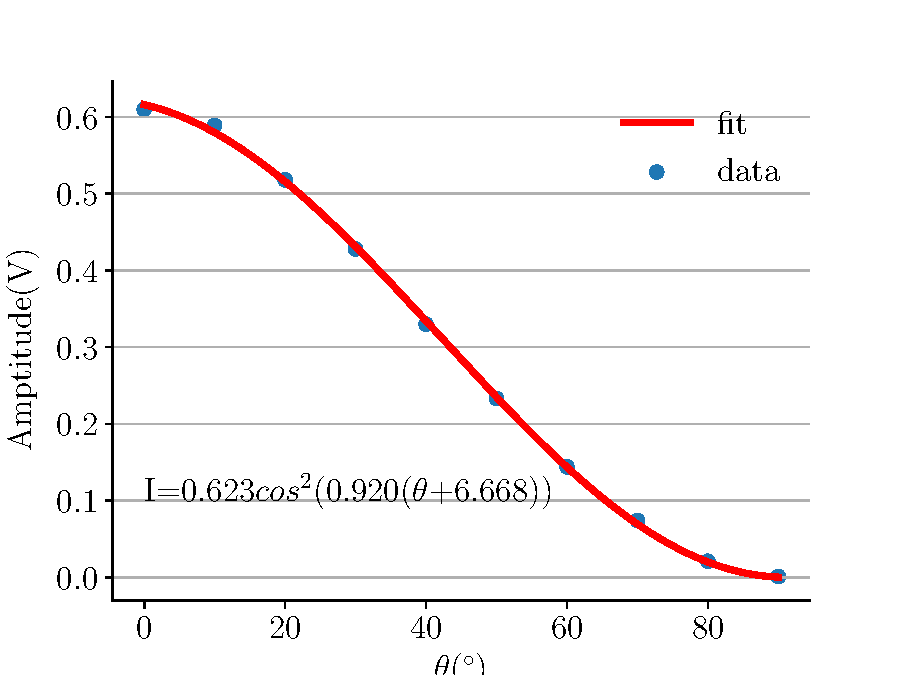
\includegraphics[width=.85\linewidth]{figure/angle.eps}
            \caption{a pciture}
        \end{figure}
    \end{multicols}
       

    \begin{tblr}{
        width = .8\textwidth,
        colspec = {XXX}
    }
        \hline
        \SetCell[r=2,c=2]{c} % 直接设置合并单元格 2行2列 水平垂直居中
        合并的格子 & ~ & % 合并后的格子必须保留 “&” 并空置
        独立的格子1 \\

        \cline{2-3}
        ~ & ~ & 独立的格子2 \\
        \hline 
    \end{tblr}

    %  \begin{longtabu}{
    %     width = .8\textwidth,
    %     colspec = {XXX}
    % }
    %     A & B & C \\
    %     1 & 2 & 3
    % \end{longtabu}

    \begin{tblr}{
        width = .9\linewidth,
        colspec = {X[1,c,m]|X[1,c,m]X[1,c,m]X[1,c,m]X[1,c,m]X[1,c,m]X[1,c,m]X[1,c,m]X[1,c,m]X[1,c,m]}
    }
    \toprule
    $I/\si{\milli\ampere}$ & 20    & 30    & 40    & 50    & 60    & 70    & 80    & 90    & 100 \\
    \midrule
    $U_2/\si{V}$ & 0.56  & 1.84  & 3.86  & 5.56  & 3.4   & 1.88  & 0.92  & 0.52  & 0.28 \\
    $U_1/\si{V}$ & 7.88  & 7.6   & 6.92  & 5.8   & 6.68  & 7     & 7.24  & 7.24  & 7.16 \\
    \bottomrule
    \end{tblr}

    % \bibliography{bibtest}
    \bibreference[nocite,style=author-year,newpage]{ref}
    
    

\end{document}

